% chap1.tex

\chapter{Introduction}\label{chap:intro}

A programming curriculum in an introductory programming syllabus requires students to learn foundational programming skills and concepts. Conventionally a programming language is taught with a Hello World example. Consider a simple problem to display “Hello World” 
on the console. Following are the programs written in three popular programming 
languages: C, Java and Python, as shown in the listing ~\ref{c}, ~\ref{java} and ~\ref{py}.

\begin{lstlisting}[language=C,caption=Hello World program in C,label=c,showstringspaces=false,columns=flexible,basicstyle={\small\ttfamily}]
#include <stdio.h>
int main() 
{
    printf("Hello World!");
    return 0;
}
\end{lstlisting}

\begin{lstlisting}[language=Java,caption=Hello World program in Java,label=java,showstringspaces=false,columns=flexible,basicstyle={\small\ttfamily}]
public class HelloWorld {
    public static void main(String[] args) {
        System.out.println("Hello World!");
    }
}
\end{lstlisting}

\begin{lstlisting}[language=Python,caption=Hello World program in Python,label=py,showstringspaces=false,columns=flexible,basicstyle={\small\ttfamily}]
print "Hello World!"
\end{lstlisting}

Each programming language presents its own set of difficulties to make it understand for a beginner. In C, the challenge for students is to understand the concepts of main, preprocessor directive, header file and return type in a first instance. The Java program too involves concepts of class, access modifier, static keyword and method call. The Python program is more intuitive  than C or Java. However the novice programmer has to remember the function to print the text. It was felt that the beginners tend to learn the intricacies of programming if they are motivated. The idea is to introduce to a set of building block functions which is easy to program and then introduce students with similar concepts in any of the programming languages mentioned above.

In this visual approach to programming, a programmer need not remember any of the constructs of a programming language, but only on the approach to solve a problem. Visual programming has been an active research area in recent years resulting in many visual programming languages. In computing, a visual programming language (VPL) is any programming language that lets users create programs by manipulating program elements graphically rather than by specifying them textually. Scratch ~\ref{fig:scratch} developed by the MIT Media Labs in 2005 is a popular visual programming language. Scratch is used by students, scholars, teachers, and parents to provide a stepping stone to the more advanced world of computer programming.

\begin{figure}[h]
\centering
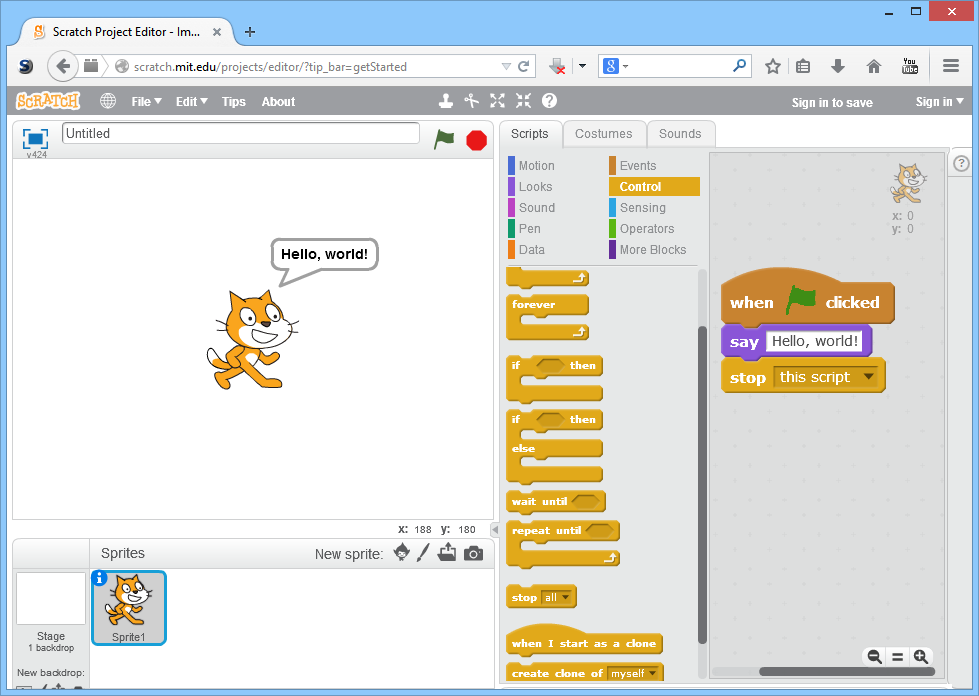
\includegraphics[width=1\columnwidth]{Images/scratch}
\caption{Hello World program in Scratch}
\label{fig:scratch}
\end{figure}

In this research, we extend the idea of using visual programming language with a real robot. This gives a platform to learn fundamentals of programming as well as robotics. 

LEGO is known for its educational robotics line through the Mindstorms robotics kit since 2006. The Education EV3 Core Set consists of EV3 programmable brick (ARM9-based processor), motors, different types of sensors and around 500 accessories. Very simple programs for the robot can be created using the programmable brick itself. For complex programs, a visual programming software is included in the package. Lego's Mindstorm kit was adopted by Department of Computer Science of US Air Force Academy~\cite{lego} to teach programming. However the LEGO kits are not affordable and the building blocks developed is not based on open source designs. The open source design implies that both hardware and software can be independently
extended if required. A similar work was done by University of Alabama Computer Science 
Department which used a 3D graphical environment Alice~\cite{alice} and iRobots for its introductory CS course~\cite{irobot}. Their course topics cover objects, methods, variables, loops, nested ifs, user input, parameters, events, random numbers, arrays and recursion. The software development was made open source, yet the hardware design was restricted
to iRobot proprietary design.

Hence a need for an economical robotic kit with an open source hardware design and software
platform is required for the beginners. The subsequent chapters disusses in detail the design and development of this interactive educational platform.



 
